\documentclass[10pt,a4paper,notitlepage]{article}
%Mise en page
\usepackage[left=2cm, right=2cm, lines=45, top=0.8in, bottom=0.7in]{geometry}
\usepackage{fancyhdr}
\usepackage{fancybox}
\usepackage{pdfpages} 
\usepackage{listings}
\renewcommand{\headrulewidth}{1.5pt}
\renewcommand{\footrulewidth}{1.5pt}
\pagestyle{fancy}
\newcommand\Loadedframemethod{TikZ}
\usepackage[framemethod=\Loadedframemethod]{mdframed}
\usepackage{tikz}
\usetikzlibrary{calc,through,backgrounds}
\usetikzlibrary{matrix,positioning}
%Desssins geometriques
\usetikzlibrary{arrows}
\usetikzlibrary{shapes.geometric}
\usetikzlibrary{datavisualization}
\usetikzlibrary{automata} % LATEX and plain TEX
\usetikzlibrary{shapes.multipart}
\usetikzlibrary{decorations.pathmorphing} 
\usepackage{pgfplots}
\usepackage{physics}
\usepackage{titletoc}
\usepackage{mathpazo} 
\usepackage{algpseudocode}
\usepackage{algorithmicx} 
\usepackage{bohr} 
\usepackage{xlop} 
\usepackage{bbding} 
\usepackage{hyperref}
%\usepackage{minibox} 
%Ecriture arabe
\usepackage{mathdesign}
\usepackage{bbding} 
\usepackage{romande} 
\lhead{
\textbf{UNIVERSIDADE DO MINHO}
}
\rhead{\textbf{TTI}
}
\chead{\textbf{Aulas PL}}

\lfoot{J. J. Almeida | Tiago Barata}
\cfoot{}
\rfoot{\textbf{$\mathsf{2023-2024}$}}
%\rfoot{\textit{Pr. $\mathcal{A}$.Kaal}}
%=====================Algo setup
\algblock{If}{EndIf}
\algcblock[If]{If}{ElsIf}{EndIf}
\algcblock{If}{Else}{EndIf}
\algrenewtext{If}{\textbf{si}}
\algrenewtext{Else}{\textbf{sinon}}
\algrenewtext{EndIf}{\textbf{finsi}}
\algrenewtext{Then}{\textbf{alors}}
\algrenewtext{While}{\textbf{tant que}}
\algrenewtext{EndWhile}{\textbf{fin tant que}}
\algrenewtext{Repeat}{\textbf{r\'ep\'eter}}
\algrenewtext{Until}{\textbf{jusqu'\`a}}
\algcblockdefx[Strange]{If}{Eeee}{Oooo}
[1]{\textbf{Eeee} "#1"}
{\textbf{Wuuuups\dots}}

\algrenewcommand\algorithmicwhile{\textbf{TantQue}}
\algrenewcommand\algorithmicdo{\textbf{Faire}}
\algrenewcommand\algorithmicend{\textbf{Fin}}
\algrenewcommand\algorithmicrequire{\textbf{Variables}}
\algrenewcommand\algorithmicensure{\textbf{Constante}}% replace ensure by constante
\algblock[block]{Begin}{End}
\newcommand\algo[1]{\textbf{algorithme} #1;}
\newcommand\vars{\textbf{variables } }
\newcommand\consts{\textbf{constantes}}
\algrenewtext{Begin}{\textbf{debut}}
\algrenewtext{End}{\textbf{fin}}
%================================
%================================

\setlength{\parskip}{1cm}
\setlength{\parindent}{1cm}
\setlength{\parskip}{0mm}
\setlength{\parindent}{10mm}

%===========================================================
\begin{document}

\begin{center}
\section*{Ficha N\textdegree 1: \textsc{Traduções ``manuais''}}
\end{center}

\subsection*{Exercício 1 - Instalação de um editor de texto}
O objetivo deste exercício é ajudar a instalar e configurar o editor de texto \href{https://www.sublimetext.com}{Sublime Text}, no entanto há liberdade de usar qualquer outro editor com o qual esteja familiarizado.
    \begin{enumerate}
        \item Após a instação, abrir o editor.
        \item Na barra de menus, selecionar Preferences > Settings. Abriram-se dois ficheiros em modo \textit{split vertical} - lado a lado. Na aba da esquerda estão as configurações por defeito da aplicação, que podem ser exploradas à medida que seja necessário, na aba da direita é para colocar as configurações do utilizador. 
        \item Na aba da direita, colocam-se as definições pretendidas:      
        \begin{figure}[h!]
            \hspace{2em}
            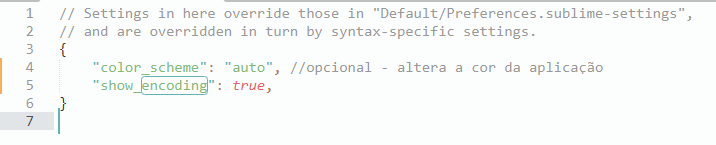
\includegraphics[width=.7\textwidth]{sublime.png}
            \label{fig:enter-label}
        \end{figure}
        \item Usar o atalho de teclado CTRL+S para guardar, ou File > Save.
    \end{enumerate}

\subsection*{Exercício 2 - Tradução manual}
O objetivo deste exercício é um pequeno exercício de tradução.
\begin{enumerate}
    \item Escolher e abrir num editor de texto um documento de teste para tradução nos \href{https://jjoao.github.io/ftt2023/materiaistextuais}{Materiais Textuais}
    \item Traduzir o texto escolhido num ficheiro à parte
\end{enumerate}

\subsection*{Exercício 3 - Tradução usando find\&replace}
O objetivo deste exercício é tentar otimizar o exercício anterior, utilizando find\&replace.
\begin{enumerate}
    \item Escolher e abrir num editor de texto o documento original do exercício anterior
    \item Procurar ocorrências de palavras repetidas na tradução (\textbf{Exemplo:} aparece muitas vezes `gato' que se traduz sempre para `cat')
    \item Após identificar todas as repetições, utiliza-se um find\&replace para substituir. Para isso usa-se o comando CTRL+H, ou Find > Replace
    \begin{figure}[h!]
        \hspace{2em}
        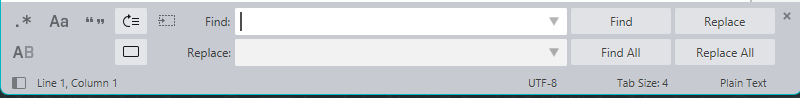
\includegraphics[width=.7\textwidth]{findreplace.png}
        \label{fig:enter-label}
    \end{figure}
    
    No campo ``Find'' coloca-se o que queremos substituir, no campo ``Replace'' coloca-se a tradução. Para aplicar, utiliza-se o botão ``Replace All''
    \item Terminar a tradução do ficheiro    
\end{enumerate}

\newpage

\subsection*{Exercício 4 - Tradução usando uma ferramenta automática}
O objetivo deste exercício é otimizar ainda mais o exercício anterior, utilizando uma ferramenta de find\&replace que pode ser descarregada \href{https://jjoao.github.io/ftt2023/util/script.py}{aqui}.
\begin{enumerate}
    \item Escolher e abrir num editor de texto o documento original do exercício anterior
    \item Procurar ocorrências de palavras repetidas na tradução (\textbf{Exemplo:} aparece muitas vezes `gato' que se traduz sempre para `cat') e guardar da seguinte maneira: 
    \begin{verbatim}
s/gato/cat/;
    \end{verbatim}
    \textit{\textbf{nota:} apenas é válida uma tradução por linha}
    \item Após a criação do ficheiro de traduções executa-se o programa, indicando o nome do ficheiro original e o de traduções. Posteriormente é criado um ficheiro de \textit{output}.
    \item Terminar a tradução do ficheiro
\end{enumerate}


\subsection*{Desafio}
No texto anterior, percebendo quais os dois sujeitos com mais ocorrências, trocá-los de posição utilizando um dos métodos do exercício 3 ou 4, por exemplo:
\begin{verbatim}
    O cão mordeu o gato.
\end{verbatim}
Passa a ser:
\begin{verbatim}
    O gato mordeu o cão.
\end{verbatim}

\end{document}